\documentclass[
    margin=1in,
    innermargin=-4.5in,
    ]{tikzposter}

% Choose size here
\geometry{paperwidth=33.11in,paperheight=46.81in} %A0
% \geometry{paperheight=33.11in,paperwidth=23.4in} %A1
    
\usepackage[utf8]{inputenc}
\usepackage{csquotes}
\usepackage{amsmath}
\usepackage{amsfonts}
\usepackage{amsthm}
\usepackage{amssymb}
\usepackage{mathrsfs}
\usepackage{graphicx}
\usepackage{lipsum}
\usepackage[export]{adjustbox}
\usepackage{tcolorbox}
\usepackage[font=small,labelfont=bf]{caption} % Required for specifying captions to tables and figures
\usepackage{enumitem}
\usepackage[backend=biber,style=numeric]{biblatex}
\usepackage{glasgow-poster-theme}
\makeatletter
\setlength{\TP@visibletextwidth}{31.0in}
\setlength{ \TP@visibletextheight}{45in}
\makeatother
\usepackage{bm}
\usepackage{bbm}

\addbibresource{refs.bib}

% set theme parameters
\tikzposterlatexaffectionproofoff
\usetheme{UniGlasgowTheme}
\usecolorstyle{UniGlasgowStyle}

\usepackage[scaled]{helvet}
\renewcommand\familydefault{\sfdefault} 
\renewcommand{\vec}[1]{\bm{#1}}
\newcommand{\Tr}{\text{Tr}}
\usepackage[T1]{fontenc}


\title{\parbox{0.8\linewidth}{\textbf{Glasgow Poster Template -}\\ \textbf{Example of a 2-line title}}}
\author{Robert Szafarczyk\textsuperscript{1}}
\institute{\textsuperscript{1}School of Computing Science, University of Glasgow}

% Adjust trim if title doesn't have two lines
\titlegraphic{
\includegraphics[width=0.35\linewidth, trim={0 2cm 0 2cm}, clip]{figures/logo_glasgow.jpg}}


% begin document
\begin{document}
\maketitle
\centering
\begin{columns}
    \column{0.5}
    \block{Problem}{
       \lipsum[30]
        
     \lipsum[10]
     
     \begin{align*}
         x = \frac{-b \pm\sqrtsign{b^2 - 4ac}}{2a}.
     \end{align*}
     
    \lipsum[20]
    }
    
    \block{Method}{
        \begin{center}
            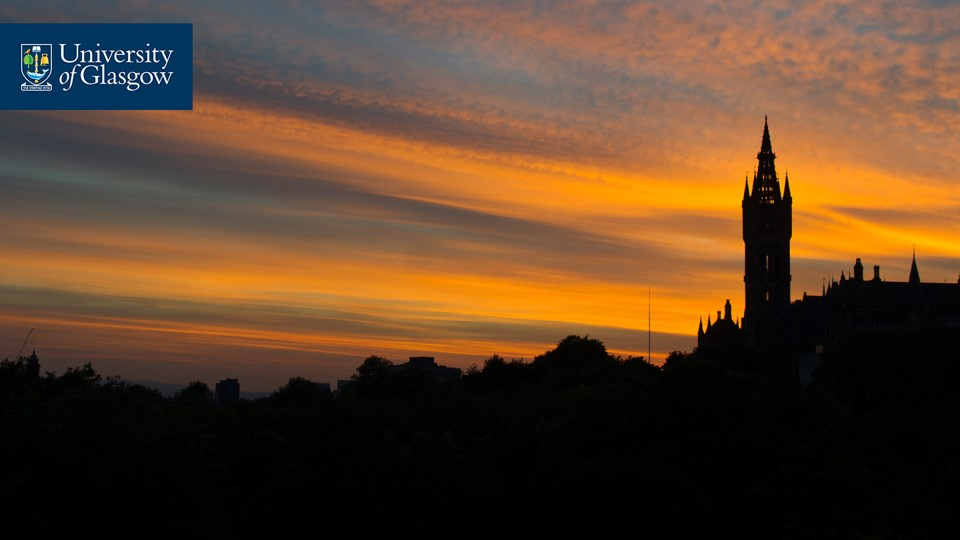
\includegraphics[width=0.8\linewidth]{figures/glasgow_sunset.jpg}
            \captionof{figure}{Sunset in Glasgow}
        \end{center}
        
        \vspace{1cm}
    
        \lipsum[100]
        \lipsum[100]
        \lipsum[100]
    }


    \column{0.5}
    \block{Evaluation}{
        \lipsum[100]
        \lipsum[100]
        \lipsum[100]
        \lipsum[100]
    }

    \block{Conclusions}{
        \lipsum[100]
        \cite{hudak2007history}
        \lipsum[100]
        \lipsum[100]
    }
    
    \block{References}{
                \begin{center}
                   \mbox{}\vspace{-1\baselineskip}
    \printbibliography[heading=none] 
        \end{center}
        }

\end{columns}
\end{document}